% Template for Cogsci submission with R Markdown

% Stuff changed from original Markdown PLOS Template
\documentclass[10pt, letterpaper]{article}

\usepackage{cogsci}
\usepackage{pslatex}
\usepackage{float}
\usepackage{caption}

% amsmath package, useful for mathematical formulas
\usepackage{amsmath}

% amssymb package, useful for mathematical symbols
\usepackage{amssymb}

% hyperref package, useful for hyperlinks
\usepackage{hyperref}

% graphicx package, useful for including eps and pdf graphics
% include graphics with the command \includegraphics
\usepackage{graphicx}

% Sweave(-like)
\usepackage{fancyvrb}
\DefineVerbatimEnvironment{Sinput}{Verbatim}{fontshape=sl}
\DefineVerbatimEnvironment{Soutput}{Verbatim}{}
\DefineVerbatimEnvironment{Scode}{Verbatim}{fontshape=sl}
\newenvironment{Schunk}{}{}
\DefineVerbatimEnvironment{Code}{Verbatim}{}
\DefineVerbatimEnvironment{CodeInput}{Verbatim}{fontshape=sl}
\DefineVerbatimEnvironment{CodeOutput}{Verbatim}{}
\newenvironment{CodeChunk}{}{}

% cite package, to clean up citations in the main text. Do not remove.
\usepackage{apacite}

% KM added 1/4/18 to allow control of blind submission
\cogscifinalcopy

\usepackage{color}

% Use doublespacing - comment out for single spacing
%\usepackage{setspace}
%\doublespacing


% % Text layout
% \topmargin 0.0cm
% \oddsidemargin 0.5cm
% \evensidemargin 0.5cm
% \textwidth 16cm
% \textheight 21cm

\title{Integrating Common Ground and Informativeness in Pragmatic Word Learning}


\author{{\large \bf Manuel Bohn} \\ \texttt{bohn@stanford.edu} \\ Psychology, Stanford University \\ LFE, Leipzig University 
 \And {\large \bf Michael Henry Tessler} \\ \texttt{tessler@mit.edu} \\ Department of Brain and Cognitive Sciences \\ Massachusetts Institute of Technology
 \And {\large \bf Michael C. Frank} \\ \texttt{mcfrank@stanford.edu} \\ Department of Psychology \\ Stanford University}

\begin{document}

\maketitle

\begin{abstract}
Pragmatic inferences are an integral part of language learning and
comprehension. To recover the intended meaning of an utterance,
listeners need to balance and integrate different sources of contextual
information. In a series of experiments, we studied how listeners
integrate general expectations about speakers with expectations specific
to their interactional history with a particular speaker. We used a
Bayesian pragmatics model to formalize the integration process. In
Experiments 1 and 2, we replicated previous findings showing that
listeners make inferences based on speaker-general and speaker-specific
expectations. We then used the empirical measurements from these
experiments to generate model predictions about how the two kinds of
expectations should be integrated, which we tested in Experiment 3.
Experiment 4 replicated and extended Experiment 3 to a broader set of
conditions. In both experiments, listeners based their inferences on
both types of expectations. We found that model performance was also
consistent with this finding; with better fit for a model which
incorporated both general and specific information compared to baselines
incorporating only one type. Listeners flexibly integrate different
forms of social expectations across a range of contexts, a process which
can be described using Bayesian models of pragmatic reasoning.

\textbf{Keywords:}
Pragmatics; Word learning; Common ground; Bayesian models
\end{abstract}

\section{Introduction}\label{introduction}

One of the most astonishing features of natural language is that it
allows us to communicate precise meanings despite the fact that most
utterances are inherently ambiguous. While the conventional mapping
between sounds (words) and objects constrain what a speaker may mean by
an utterance, the intended meaning of the utterance is not reducible to
the words that are contained in it. It takes additional pragmatic
inference to recover the intended meaning (Levinson, 2000).

Pragmatic inferences rest on a set of expectations that interlocutors
bring to the table when entering a communicative interaction. On the one
hand, speakers and listeners have the general expectation that their
partner communicates in an informative and relevant way (Sperber \&
Wilson, 2001). Grice (1991) summarised this expectation via the
\emph{Cooperative Principle}: ``Make your contribution such as is
required, at the stage at which it occurs, by the accepted purpose or
direction of the talk exchange in which you are engaged.'' Importantly,
the second half of the Cooperative Principle describes a second type of
expectation: interlocutors expect each other to produce and interpret
utterances \emph{in light of the shared common ground between them} (H.
H. Clark, 1996). Common ground refers to bits of information that are
assumed to be shared, either because they were mentioned over the course
of the conversation or grounded through some form of joint experience
(Bohn \& Koymen, 2018). Note that by its very nature, common ground may
vary with the individuals involved in a particular conversation.

These same general and specific expectations can support children's word
learning (E. V. Clark, 2009; Tomasello, 2009). On the one hand, children
have been found to learn novel words by assuming speakers are generally
informative (Frank \& Goodman, 2014). That is, in the absence of any
prior interaction with the speaker, children interpreted a novel word as
referring to the most informative referent. On the other hand, children
use conversation-specific common ground expectations to decide which
object a specific speaker is referring to when they use a novel word
(Akhtar, Carpenter, \& Tomasello, 1996). For example, when a speaker
expressed preference for a particular object, children expect a novel
word from the same speaker to refer to the previously preferred object
(Saylor, Sabbagh, Fortuna, \& Troseth, 2009).

But how do listeners integrate general and common ground-related
expectations during word learning? Are pragmatic inferences strengthened
additively when both support a particular interpretation? How are they
weighed when they are in conflict? The Rational Speech Act (RSA)
framework (Frank \& Goodman, 2012; Goodman \& Frank, 2016) offers a
formal framework for addressing this information integration problem.
RSA models are characterized by a recursive structure in which a
pragmatic listener tries to uncover a speaker's intended meaning by
assuming the speaker chose their utterance in order to get a naive
listener to recover their intended meaning. RSA models have made
accurate quantitative predictions about various forms of pragmatic
language use and word learning (Goodman \& Frank, 2016). However, a
comprehensive treatment of how general and common ground expectations
are integrated is still missing.

Within RSA models, each agent in the recursion is modeled as a Bayesian
reasoner; thus, information integration is treated as a process of
probabilistic inference. The speaker-general informativeness expectation
is already encoded in the structure of the model: Speakers produce
utterances to aid the listener in disambiguating referents. We
operationalize speaker-specific, common ground information as the shared
prior probability of referents in the context of the utterance. Thus, a
natural locus for information integration within these models is the
trade off between the prior probability of a particular referent and the
likelihood of that referent given the current utterance.

Here we evaluate this rational, pragmatic account of information
integration. We isolate speaker-specific and common-ground information
experimentally, then test how adult listeners combine them in a word
learning setting. In Experiments 1 and 2, we replicate findings showing
that listeners expect speakers to a) produce informative utterances
(Experiment 1) and b) communicate about things that are relevant to
common ground (Experiment 2). Based on these results, we generate model
predictions using the RSA framework about how these two components
should be integrated. In Experiment 3, we test how listeners integrate
their expectations and compare model predictions to empirical data.
Experiment 4 replicates and extends Experiment 3 by varying the strength
of common ground assumptions. For all experiments, we pre-registered the
sample size, experimental design and the statistical analysis. For
Experiment 3 and 4, we also registered the model structure and
predictions (see {[}masked for peer review{]})

\section{Method}\label{method}

\subsection{General Design}\label{general-design}

Experiments were conducted online using Amazon's Mechanical Turk. Fig.
\ref{fig:design} provides a schematic overview of the setup and
experimental procedures. The instructions informed participants that
they would see a number of animal characters asking for novel toys.
Participants were asked to identify the toy being requested by a
particular animal. The basic layout involved two tables with toys on
them, located left and right of a little hill, on which the animal was
standing. For each animal, we recorded a set of utterances (one speaker
per animal) that were used throughout the experiments to provide
information and make requests. At test, toys were requested using the
following utterance: ``Oh cool, there is a {[}non-word{]} on the table,
how neat, can you give me the {[}non-word{]}?''. Participants responded
by clicking on one of the toys. Each experiment started with two
training trials in which animals requested familiar objects (car and
ball).

\begin{CodeChunk}
\begin{figure*}[h]

{\centering 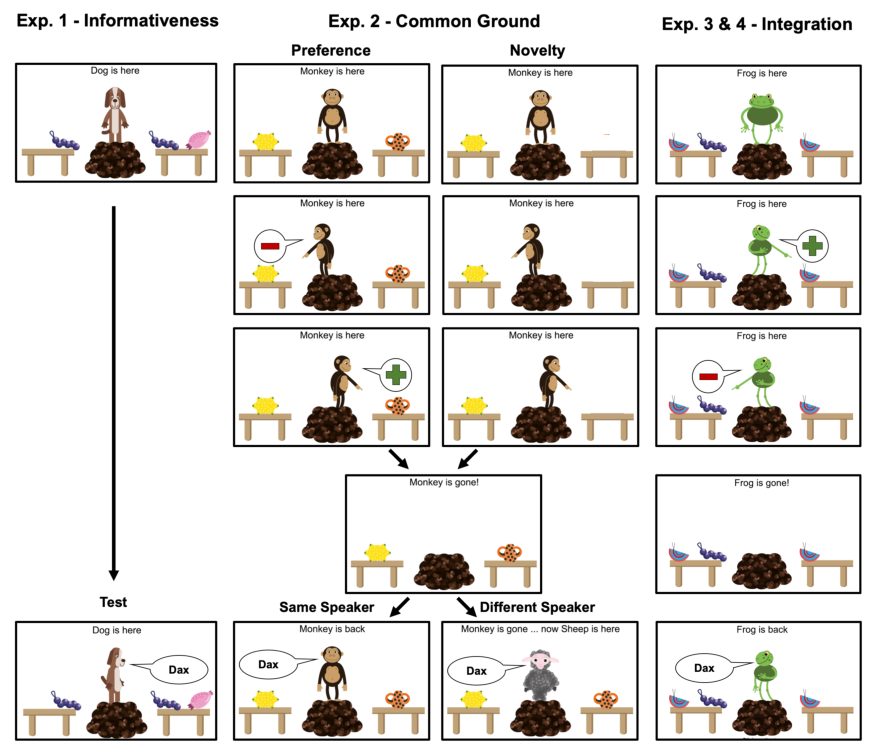
\includegraphics{figs/design-1} 

}

\caption[Schematic experimental procedure]{Schematic experimental procedure. In all conditions, at test (bottom), the speaker ambiguously requested an object using a non-word (e.g. “dax”). Participants clicked on the object they thought the speaker referred to. Informativeness (Experiment 1, left) translated to making one object less frequent in context. Common ground (Experiment 2, middle) was manipulated by making one object prefered by or new to the speaker. Green plus signs represent utterances that expressed preference and red minus of dispreference (see main text for details). Experiment 3 (right) combined manipulations. When expressing e.g. preference for an object on a table with two objects (panel 3 from top), the respective object was temporarily enlarged. Condition for Experiment 3 shown here: preference - same speaker - incongruent.}\label{fig:design}
\end{figure*}
\end{CodeChunk}

\section{Experiment 1}\label{experiment-1}

\subsection{Participants, Design and
Procedure}\label{participants-design-and-procedure}

All participants were recruited from Amazon Mechanical Turk and had US
IP addresses. Sample size in each experiment was planned to be 120 data
points per cell. Experiment 1 had 40 participants. In the test
condition, one table contained one object of type A and the other table
contained one object of type A and one of type B (see Fig.
\ref{fig:design}, left). On each trial, the animal introduced themselves
(e.g. ``Hi, I'm Dog''), turned towards the table with the two objects
and made a request. If listeners expect speakers to produce informative
utterances, they should select object B. This choice follows from the
counterfactual inference that if the (informative) speaker would have
wanted to request A, they would have turned to the table that only
contained A. On the other hand, since B is only located on the table
together with A, there was no alternative way to request B in a less
ambiguous way. In the control condition, both tables contained two
objects, one of which was randomly determined as the correct one. No
inference was therefore licensed. Each participant received three trials
in each condition for a total of six trials, presented in a randomized
order.

\subsection{Results and Discussion}\label{results-and-discussion}

Participants selected the less frequent object above chance in the test
condition (t(39) = 5.51, \emph{p} \textless{} .001, see Fig.
\ref{fig:plotexp12}) and did so more often compared to the control
condition (generalized linear mixed model
(GLMM\footnote{All models had maximal random effects structure conditional on model convergence.}):\emph{\(\beta\)}
= 1.28, se = 0.29 \emph{p} \textless{} .001). This result replicates
earlier work (Frank \& Goodman, 2014) and is consistent with the
hypothesis that listeners expect speakers to communicate in an
informative way.

\begin{CodeChunk}
\begin{figure}[H]

{\centering 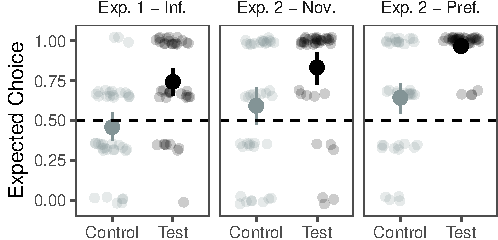
\includegraphics{figs/plotexp12-1} 

}

\caption[Results from Experiment 1 and 2]{Results from Experiment 1 and 2. For preference and novelty, control refers to a different speaker (see Fig. 1). Transparent dots show data from individual participants, solid dots represent condition means, error bars are 95\% CIs. Dashed line indicates performance expected by chance.}\label{fig:plotexp12}
\end{figure}
\end{CodeChunk}

\section{Experiment 2}\label{experiment-2}

We manipulated common ground expectations based on procedures that have
successfully been used in developmental studies (e.g. Akhtar et al.,
1996; Saylor et al., 2009). Speakers either expressed preference for one
object or one object was new to the speaker.

\subsection{Participants, Design and
Procedure}\label{participants-design-and-procedure-1}

We collected data from 80 participants, with 40 in each condition. In
the preference condition, each table had a different object. In the
beginning, the animal appeared on the hill and introduced themselves.
Next, they turned to one of the tables and expressed either that they
liked (``Oh wow, I really like that one'') or disliked (``Oh bleh, I
really don't like that one'') the object before turning to the other
side and expressing the respective other attitude. Then, the animal
disappeared. After a short period of time, either the same or a
different animal appeared and requested an object while facing straight
ahead (see Fig. \ref{fig:design}, middle). If participants took into
account the information they gained about the speaker, they should
select the previously preferred object if the returning animal was the
same. If a different animal returned, they should choose randomly
between objects.

In the novelty condition, one table was initially empty while there was
an object on the other table (see Fig. \ref{fig:design}). The animal
turned to one of the sides and commented either on the presence (``Aha,
look at that'') or the absence of an object (``Hm, nothing there'').
Next, the animal disappeared. The same animal re-appeared and the
sequence above was repeated. When the animal disappeared for the second
time, a second object appeared on the empty table while the animal was
away. Like in the preference condition, we now manipulated if the same
animal or a different one returned. In case of the same animal
returning, listeners could infer the referent of the subsequent request
by considering that one object was new to the speaker and therefore more
likely to be of interest to them. However, no such inference was
licensed when a different animal returned because both objects were
novel.

\subsection{Results and Discussion}\label{results-and-discussion-1}

Participants selected the preferred object above chance when the same
animal returned (t(39) = 29.14, \emph{p} \textless{} .001, see Fig.
\ref{fig:plotexp12}) and did so more often compared to trials in which a
different animal returned (GLMM: \(\beta\) = 2.92, se = 0.56, \emph{p}
\textless{} .001). Thus, listeners inferred the referent of the
utterance by considering previous interactions with the speaker.
Interestingly, participants transferred preference to some extent from
one animal to the other and selected the preferred object above chance
when a different animal returned (t(39) = 2.7, \emph{p} = .01). In sum,
this study shows that adults make comparable inferences to children
(Saylor et al., 2009).

The novel object was selected above chance when the same animal returned
(t(39) = 6.77, \emph{p} \textless{} .001) but not when a different one
appeared (t(39) = 1.49, \emph{p} = .144, see Fig. \ref{fig:plotexp12}).
Furthermore, the two conditions differed in the expected direction
(\(\beta\) = 6.27, se = 1.96, \emph{p} = .001). Thus, like children
(Akhtar et al., 1996), adults used their prior information about the
speaker to resolve ambiguity in the utterance.

\section{Experiment 3}\label{experiment-3}

\begin{CodeChunk}
\begin{figure*}[h]

{\centering 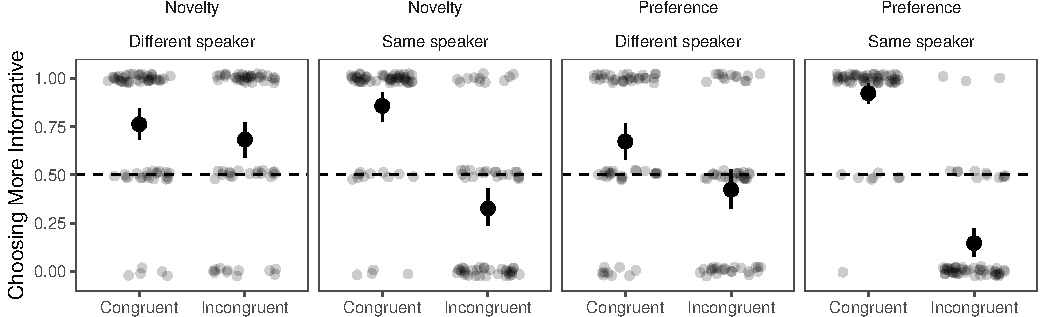
\includegraphics{figs/plotexp3-1} 

}

\caption[Results from Experiment 3]{Results from Experiment 3. Dashed line indicates performance expected by chance. Plotting conventions are the same as in Fig. 2. All conditions in which CIs do not overlap with chance line are also statistically different from chance based on two-tailed Wilcoxon tests.}\label{fig:plotexp3}
\end{figure*}
\end{CodeChunk}

In Experiment 3, we combined the expectations studied in Experiment 1
and 2 to see how listeners integrate them.

\subsection{Participants, Design and
Procedure}\label{participants-design-and-procedure-2}

A total of 121 individuals participated in the experiment. The test
situation was the same as in the test condition in Experiment 1 (see
Fig. \ref{fig:design}, right): One table with object of type A and the
other with an object of type A and B. Again, the animal always turned to
the table with two objects and ambiguously requested an object. In
Experiment 1, the listener had no prior information about each object.
In Experiment 3, however, we manipulated common ground expectations in
the same way as in Experiment 2. For example, the animal would turn to
the table with one object and express that they don't like object A,
then turn to the other table and express that they like object B. Next,
after quickly disappearing, they would reappear, turn to the table with
two objects and make a request.

For each common ground condition, there were 4 conditions in Experiment
3 resulting from the cross of congruent/incongruent informativeness with
same/different speaker. If the preferred/novel object was the less
frequent one (object B), the two expectations were congruent. If the
preferred/novel object was the more frequent one (object A),
expectations were incongruent. For each type of expectation alignment,
we varied if the same or a different animal returned. Participants
either completed the preference or novelty version with two test trials
in each of the four conditions. Before discussing the empirical results,
we briefly discuss the model we used to predict expectation integration.

\subsection{Model Predictions}\label{model-predictions}

To derive predictions, we used a probabilistic RSA model that simulates
a pragmatic listener reasoning about a cooperative speaker who is trying
to refer to an object (Frank \& Goodman, 2012). The speaker chooses how
to refer to the object by reasoning about a naive listener who does not
know the labels for the object (Frank \& Goodman, 2014). The conditional
probability that the listener chooses a referent given an utterance is
defined as follows: \[P_L(r_s|u)\propto P_S(u|r_s)P_S(r_s)\] Here,
\(P_S(u|r_s)\) is the likelihood that the speaker will use an utterance
\(u\) to refer to a specific referent r. It is defined in terms of a
utility function \(U_S(u;s)\) consisting of the surprisal of \(u\) for a
naive listener \(L_0\), who interprets \(u\) according its literal
semantics: \[P_S(u|r_s)\propto exp(\alpha U_S(u;s))\] The numerical
strength of the expression above depends on a scalar value, \(\alpha\),
which can be interpreted as an indicator of how rational the speaker is
in choosing utterances (i.e.~as \(\alpha\) increases, the speaker is
more likely to choose the most informative utterance).

The term \(P_S(r_s)\) denotes the prior probability that a speaker will
refer to a given referent. This probability represents the listeners
expectations about the speaker depending on the manipulation (preference
or novelty) and the identity of the speaker (same or different speaker).

We used the results from Experiment 1 and 2 to specify \(\alpha\) as
well as \(P_S(r_s)\) in our model. We set \(\alpha\) so that a model
with uniform priors would predict the average proportion measured in
Experiment 1. The prior probability for each object was set to be the
proportion with which this object was chosen in Experiment
2\footnote{Proportions were measured when participants chose between two objects. However, in Experiment 3, three objects were involved. For each object we used the proportion measured in Experiment 2 as the prior probability.This approached spread out the absolute probability mass for each object but conserved the relative relation between objects.}.
Based on these parameter settings, we predicted the proportion with
which listeners will choose the more informative object in each of eight
unique conditions mentioned above (see also Fig. \ref{fig:plotexp3}). We
compared the fit of this pragmatic model to two alternative models using
Bayes Factors (BF). The first alternative model ignored the speaker
specific expectations (uniform prior model) while the second ignored the
informativeness inference (prior only model). All models included a
noise parameter, reflecting that participants may respond randomly
instead of in line with the intended manipulation on a given trial.
Noise parameters were estimated based on the data. They range between 0
and 1 and reflect the proportion of responses that are estimated to be
random instead of following the pattern predicted by the model.

\subsection{Results and Discussion}\label{results-and-discussion-2}

Results are discussed in the form of the proportion with which listeners
chose the more informative object (i.e., the object that would be the
more informative referent when only considering speaker general
expectations). For a comparison to chance within each unique condition
see Fig. \ref{fig:plotexp3}. Combinations of alignment and speaker
identity differed in how they influenced participants' responses (GLMM
model term: \texttt{alignment*speaker}; \(\beta\) = -2.64, se = 0.48,
\emph{p} \textless{} .001). Fig. \ref{fig:plotmodelcomp}A shows the mean
response in each unique condition compared to the pragmatics model.
Model predictions and data were highly correlated (r = 0.96, \emph{p}
\textless{} .001). Model fit was much better in the model taking into
account both types of expectations compared to the uniform prior (BF =
2e+79) or prior only model (BF = 1.8e+34). The inferred noise level in
the pragmatics model was 0.27 (95\% HDI: 0.21 - 0.34).

Interestingly, as in Experiment 2, there was a transfer of preference in
the case of speaker change. Participants were at chance in the
preference - different speaker - incongruent condition (see Fig.
\ref{fig:plotexp3}). If preference would have been specific to a
particular individual, participants should have selected the less
frequent object above chance (as they did in the corresponding condition
with the novelty manipulation). Because it takes into account the
measurement from the earlier experiment, our model predicts these
results; future work might explicitly model generalization across
speakers.

\section{Experiment 4}\label{experiment-4}

Here we replicated and extended Experiment 3 by manipulating the
strength of the common ground expectations.

\subsection{Participants, Design and
Procedure}\label{participants-design-and-procedure-3}

This experiment had 453 participants. The structure of the experiment
was the same as in Experiment 3. For each common ground expectation
(preference and novelty), we intended to have a strong, a medium and a
weak condition. The strength of each condition was determined by the
proportion with which participants chose the preferred/novel object
given the manipulation. We succeeded in generating quantitative
variability for novelty. For preference we piloted a number of
additional manipulations but did no find one that yielded a weaker
preference compared to a medium condition.

The strong manipulations were identical to Experiment 3 and the results
are therefore a direct replication (see Fig. \ref{fig:plotmodelcomp}C).
For novelty, in the medium condition, the animal turned to each table
only once before the test. In the weak condition, the animal only turned
to the table with an object before the test (instead of turning to and
commenting on both). In the medium condition for preference, the animal
only expressed liking and did so in a more subtle way (saying only:
``Oh, wow'' while pointing to the object). Participants were assigned to
one level of common ground expectation and completed two test trials in
each of the four conditions (alignment x speaker change).

Model predictions were obtained in the same way as in Experiment 3; with
\(\alpha\) inferred from the data and \(P_S(r_s)\) measured empirically
(in a set of corresponding experiments parallel to Experiment 2).

\subsection{Results and Discussion}\label{results-and-discussion-3}

\begin{CodeChunk}
\begin{figure*}[h]

{\centering 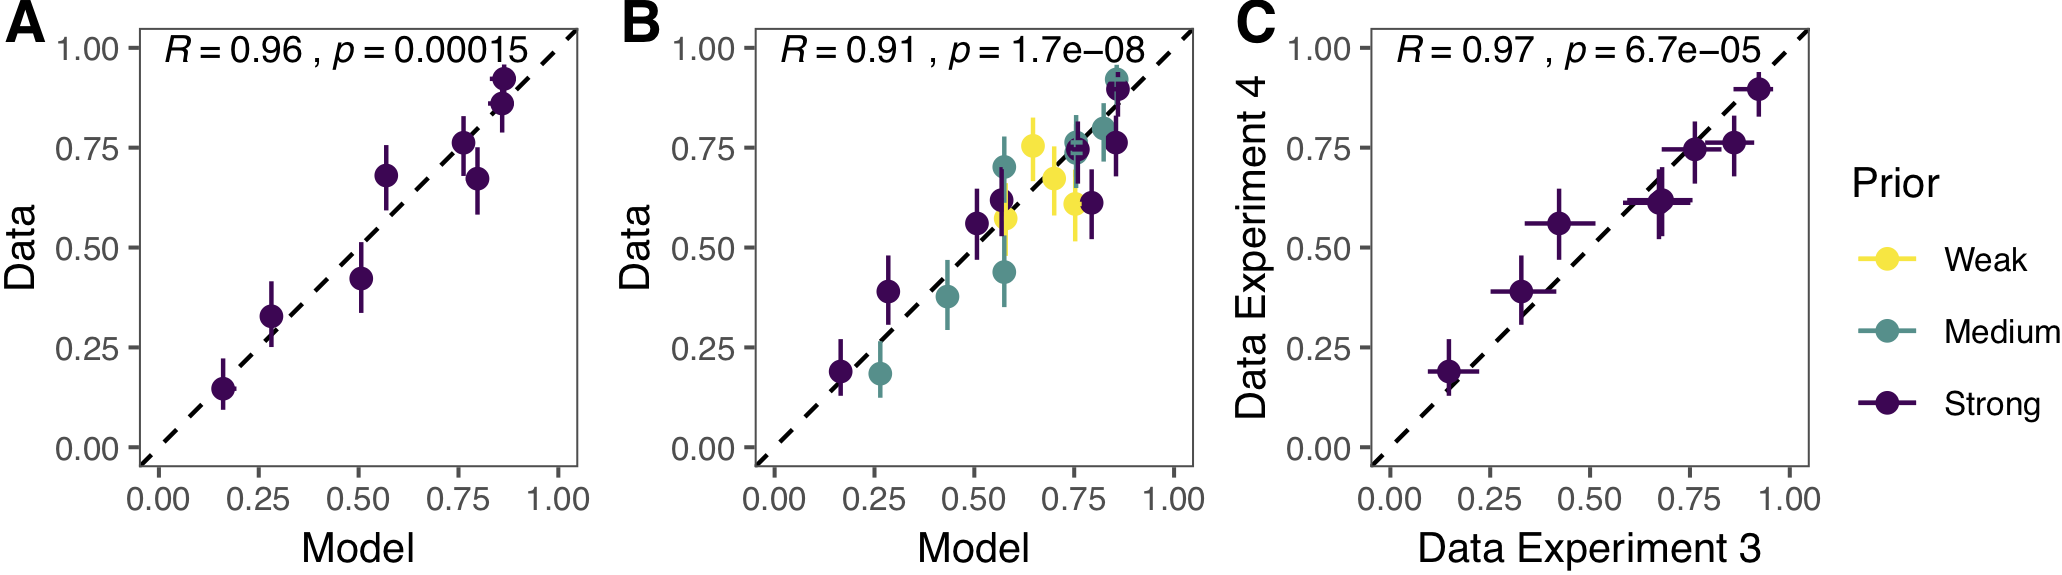
\includegraphics{figs/plotmodelcomp-1} 

}

\caption[(A) Model predictions compared to data for Experiment 3 and (B) Experiment 4]{(A) Model predictions compared to data for Experiment 3 and (B) Experiment 4. (C) Data for strong prior manipulation in Experiment 3 and 4, providing a noise ceiling for the reliability of measurements. Error bars = 95\% HDIs.}\label{fig:plotmodelcomp}
\end{figure*}
\end{CodeChunk}

As noted above, the strong prior condition was a direct replication of
Experiment 3. Results from the two rounds of data collection were highly
correlated (r = 0.97, \emph{p} \textless{} .001, see Fig.
\ref{fig:plotmodelcomp}C). Across levels of prior manipulation, the data
from Experiment 4 were highly correlated to the corresponding model
predictions (r = 0.91, \emph{p} \textless{} .001, see Fig.
\ref{fig:plotmodelcomp}B). Again, the pragmatics model provided a much
better fit compared to the flat prior (BF = 4.4e+74) or prior only model
(BF = 1.8e+84). The inferred noise level in the pragmatics model was
0.28 (95\% HDI: 0.24 - 0.32).

\section{Discussion}\label{discussion}

Language use and learning requires balancing different types of
expectations about one's interlocutor - expectations about how speakers
behave in general and expectations about how a particular speaker might
behave in a particular context. Here we used a Bayesian pragmatics model
to predict this integration process. Experiment 1 and 2 replicated
previous studies showing that adult listeners expect speakers to produce
utterances informatively and also with respect to common ground. We then
combined the procedures from the first two experiments to study how
listeners would integrate expectations. We used the results from
Experiment 1 and 2 to specify model parameters that represented the two
types of expectations, generating predictions about new behavior.
Experiments 3 and 4 showed that both types of expectations influenced
listeners inferences. Overall, listener behavior was accurately
described by our model, suggesting that listeners trade-off flexibly
between speaker specific and general pragmatic expectations.

Notably, Experiment 3 also included situations in which the two
expectations were in conflict. For example, in some trials the speaker
expressed preference for object A, which was also the more frequent
(less informative) object. In these situations, a majority of
participants chose the preferred object as the referent (see also Fig.
\ref{fig:plotexp3} preference--same speaker--incongruent). A simple
explanation for this pattern might be that common ground manipulations
were simply ``stronger'', corroborated by the fact they produced higher
rates of expected choice than the informativeness expectation when the
two were presented in isolation (see Fig. \ref{fig:plotexp12}). In
Experiment 4, however, the medium manipulation for novelty yielded
numerically weaker results compared to the informativeness expectation
in Experiment 1, and yet participants still selected the novel object
above chance when the expectations were in conflict. Why is this?
Because common ground is represented in our model as the listener's
prior distribution, speakers can reason about it in choosing their
utterance. That is, in the mind of the listener, the speaker computes
the effect of each utterance on a naive listener with shared common
ground. Therefore, when prior interactions implicate one object as the
more likely referent, the speaker reasons that this object will be the
inferred referent of any semantically plausible utterance, even when the
same utterance would point to a different object in the absence of prior
information.

A range probabilistic frameworks been used to model word learning (e.g.
Fazly, Alishahi, \& Stevenson, 2010; Frank, Goodman, \& Tenenbaum, 2009;
Xu \& Tenenbaum, 2007). RSA models differ from other approaches in that
they treat word learning as the outcome of a social reasoning process.
In contrast to models for cross-situational word learning (Fazly et al.,
2010; Frank et al., 2009), RSA models show how learning might occur in a
one shot scenario based on pragmatic reasoning alone. While the ad hoc
informativeness inference characteristic for RSA would be predicted by
the model of Xu and Tenenbaum (2007), in their work it follows from the
``size principle'' of generalization (Tenenbaum \& Griffiths, 2001) and
not from social reasoning. In cotrast to RSA, this approach does not
offer a straightforward way to incorporate other types of social
information such as expectations following from common ground.

We treated common ground expectations as equivalent to more basic
manipulations of contextual salience (e.g.~in Frank \& Goodman, 2012)
and did not explicitly model the social-cognitive processes that give
rise to these expectations. The interaction around the object prior to
the test event simply increased the probability that this particular
speaker will refer to the object subsequently. The same change could be
brought about if one of the objects would be made perceptually more
salient, for example by making it flash. In future work, it would be
interesting to explore ways to model common ground expectations
explicitly as well as to contrast perceptual and interactional salience.

Our work integrates different perspectives on the study of pragmatic
inference. Previous work focused either on general or speaker specific
expectations. The methodological approach taken here illustrates how
computational and experimental approaches can be used in conjunction to
explicate theories of language use and learning.

\vspace{1em}
\fbox{\parbox[b][][c]{7.3cm}{\centering Corresponding data and code are available at\ \url{https://github.com/manuelbohn/mcc}}}
\vspace{1em}

\section{Acknowledgements}\label{acknowledgements}

MB received funding from the European Union's Horizon 2020 research and
innovation programme under the Marie Sklodowska-Curie grant agreement No
749229.

\section{References}\label{references}

\setlength{\parindent}{-0.1in} \setlength{\leftskip}{0.125in} \noindent

\hypertarget{refs}{}
\hypertarget{ref-akhtar1996role}{}
Akhtar, N., Carpenter, M., \& Tomasello, M. (1996). The role of
discourse novelty in early word learning. \emph{Child Development},
\emph{67}(2), 635--645.

\hypertarget{ref-bohn2018common}{}
Bohn, M., \& Koymen, B. (2018). Common ground and development.
\emph{Child Development Perspectives}, \emph{12}(2), 104--108.

\hypertarget{ref-clark2009first}{}
Clark, E. V. (2009). \emph{First language acquisition}. Cambridge:
Cambridge University Press.

\hypertarget{ref-clark1996using}{}
Clark, H. H. (1996). \emph{Using language}. Cambridge: Cambridge
University Press.

\hypertarget{ref-fazly2010probabilistic}{}
Fazly, A., Alishahi, A., \& Stevenson, S. (2010). A probabilistic
computational model of cross-situational word learning. \emph{Cognitive
Science}, \emph{34}(6), 1017--1063.

\hypertarget{ref-frank2012predicting}{}
Frank, M. C., \& Goodman, N. D. (2012). Predicting pragmatic reasoning
in language games. \emph{Science}, \emph{336}(6084), 998--998.

\hypertarget{ref-frank2014inferring}{}
Frank, M. C., \& Goodman, N. D. (2014). Inferring word meanings by
assuming that speakers are informative. \emph{Cognitive Psychology},
\emph{75}, 80--96.

\hypertarget{ref-frank2009using}{}
Frank, M. C., Goodman, N. D., \& Tenenbaum, J. B. (2009). Using
speakers' referential intentions to model early cross-situational word
learning. \emph{Psychological Science}, \emph{20}(5), 578--585.

\hypertarget{ref-goodman2016pragmatic}{}
Goodman, N. D., \& Frank, M. C. (2016). Pragmatic language
interpretation as probabilistic inference. \emph{Trends in Cognitive
Sciences}, \emph{20}(11), 818--829.

\hypertarget{ref-grice1991studies}{}
Grice, H. P. (1991). \emph{Studies in the way of words}. Cambridge, MA:
Harvard University Press.

\hypertarget{ref-levinson2000presumptive}{}
Levinson, S. C. (2000). \emph{Presumptive meanings: The theory of
generalized conversational implicature}. Cambridge, MA: MIT press.

\hypertarget{ref-saylor2009preschoolers}{}
Saylor, M. M., Sabbagh, M. A., Fortuna, A., \& Troseth, G. (2009).
Preschoolers use speakers' preferences to learn words. \emph{Cognitive
Development}, \emph{24}(2), 125--132.

\hypertarget{ref-sperber2001relevance}{}
Sperber, D., \& Wilson, D. (2001). \emph{Relevance: Communication and
cognition} (2nd ed.). Cambridge, MA: Blackwell Publishers.

\hypertarget{ref-tenenbaum2001generalization}{}
Tenenbaum, J. B., \& Griffiths, T. L. (2001). Generalization,
similarity, and bayesian inference. \emph{Behavioral and Brain
Sciences}, \emph{24}(4), 629--640.

\hypertarget{ref-tomasello2009constructing}{}
Tomasello, M. (2009). \emph{Constructing a language}. Cambridge, MA:
Harvard University Press.

\hypertarget{ref-xu2007word}{}
Xu, F., \& Tenenbaum, J. B. (2007). Word learning as bayesian inference.
\emph{Psychological Review}, \emph{114}(2), 245.

\bibliographystyle{apacite}


\end{document}
